\documentclass[xcolor=tex,dvipsnames]{beamer}  
\mode<presentation>
{
  \usetheme{Singapore}
  % or ...
  \setbeamercovered{transparent}
  % or whatever (possibly just delete it)
}

\setbeamercolor{block body}{fg=black, bg=green!10}

\usepackage{fontspec} 
\usepackage[mathscr]{euscript} 
%\usepackage[xcharter]{newtxmath}
%\setmainfont{XCharter}
\setmonofont{DejaVu Sans Mono}[Scale=MatchLowercase] % provides unicode characters 


\usefonttheme{professionalfonts}
%\usepackage[english]{babel}
% or whatever
%\usepackage[latin1]{inputenc}
% or whatever
%\usepackage{times}
\usepackage[T1]{fontenc}
% Or whatever. Note that the encoding and the font should match. If T1
% does not look nice, try deleting the line with the fontenc.

%%%%%%%%%%%%%%%%%%%%%% start my preamble %%%%%%%%%%%%%%%%%%%%%%
\renewcommand{\insertnavigation}[1]{}

\addtobeamertemplate{navigation symbols}{}{%
    \usebeamerfont{footline}%
    \usebeamercolor[fg]{footline}%
    \hspace{1em}%
    \insertframenumber/\inserttotalframenumber
    \vspace{0.5em}
}

\setbeamercolor{footline}{fg=blue}
\setbeamerfont{footline}{series=\bfseries}

%\setbeamertemplate{mini frames}{}

%\usepackage{adjustbox}
\usepackage{graphicx}
\usepackage{amsmath, amssymb, amsthm}
\usepackage{mathtools}

\usepackage{fancyvrb}

\usepackage{hyperref}

\usepackage{mathrsfs} % fonts, caligraphic
\usepackage{bbm}

% tikz
\usepackage{tikz}
\usepackage{tikz-cd}
\usetikzlibrary{positioning}
\usetikzlibrary{arrows}
\usetikzlibrary{calc}
\usetikzlibrary{intersections}
\usetikzlibrary{matrix}
\usetikzlibrary{decorations}
\usetikzlibrary{shapes, fit}
\usetikzlibrary{arrows.meta}
\usetikzlibrary{decorations.pathreplacing}  %for brac

\usepackage{pgf}
\usepackage{pgfplots}
\pgfplotsset{compat=1.7}


\usepackage{graphviz}

%\usepackage[usenames, dvipsnames]{color}


% nice inequalities
\renewcommand{\leq}{\leqslant}
\renewcommand{\geq}{\geqslant}


\setlength{\parskip}{1.5ex plus0.5ex minus0.5ex}
\setlength{\jot}{12pt} 

\usepackage[ruled, lined]{algorithm2e}


\definecolor{pale}{RGB}{235, 235, 235}
\definecolor{pale2}{RGB}{175,238,238}
\definecolor{turquois4}{RGB}{0,134,139}
\definecolor{DarkOrange1}{RGB}{255,127,0}

\newcommand{\emp}[1]{\textcolor{DarkOrange1}{\bf #1}}
\newcommand{\newtopic}[1]{\textcolor{Green}{\Large \bf #1}}
\newcommand{\navy}[1]{\textcolor{Blue}{\bf #1}}
\newcommand{\navymth}[1]{\textcolor{Blue}{#1}}
\newcommand{\red}[1]{\textcolor{red}{#1}}

% Minted
\definecolor{bg}{rgb}{0.95,0.95,0.95}
\usepackage{minted}
\usemintedstyle{friendly}
\newminted{python}{mathescape,frame=lines,framesep=4mm,bgcolor=bg}
\newminted{ipython}{mathescape,frame=lines,framesep=4mm,bgcolor=bg}
\newminted{julia}{mathescape,frame=lines,framesep=4mm,bgcolor=bg}
\newminted{c}{mathescape,frame=lines,framesep=4mm,bgcolor=bg}
\renewcommand{\theFancyVerbLine}{\sffamily
    \textcolor[rgb]{0.5,0.5,1.0}{\scriptsize {\arabic{FancyVerbLine}}}}


\definecolor{Brown}{rgb}{0.59, 0.29, 0.0}
\newcommand{\Fact}{\textcolor{Brown}{\bf Fact. }}
\newcommand{\Thm}{\textcolor{Brown}{\bf Theorem. }}
\newcommand{\Eg}{\textcolor{ForestGreen}{Example. }}
\newcommand{\Egs}{\textcolor{ForestGreen}{Examples. }}
\newcommand{\Ex}{{\bf Ex. }}

\newcommand{\CC}{\mathbbm C}
\newcommand{\EE}{\mathbbm E}
\newcommand{\FF}{\mathbbm F}
\newcommand{\RR}{\mathbbm R}
\newcommand{\KK}{\mathbbm K}
\newcommand{\MM}{\mathbbm M}
\newcommand{\NN}{\mathbbm N}
\newcommand{\PP}{\mathbbm P}
\newcommand{\TT}{\mathbbm T}
\newcommand{\QQ}{\mathbbm Q}
\newcommand{\WW}{\mathbbm W}
\newcommand{\VV}{\mathbbm V}
\newcommand{\ZZ}{\mathbbm Z}

\newcommand{\Asf}{\mathsf A}
\newcommand{\Esf}{\mathsf E}
\newcommand{\Fsf}{\mathsf F}
\newcommand{\Gsf}{\mathsf G}
\newcommand{\Msf}{\mathsf M}
\newcommand{\Lsf}{\mathsf L}
\newcommand{\Nsf}{\mathsf N}
\newcommand{\Psf}{\mathsf P}
\newcommand{\Qsf}{\mathsf Q}
\newcommand{\Ssf}{\mathsf S}
\newcommand{\Tsf}{\mathsf T}
\newcommand{\Xsf}{\mathsf X}
\newcommand{\Ysf}{\mathsf Y}
\newcommand{\Vsf}{\mathsf V}
\newcommand{\Wsf}{\mathsf W}
\newcommand{\Zsf}{\mathsf Z}

\newcommand{\aA}{\mathscr A}
\newcommand{\bB}{\mathscr B}
\newcommand{\cC}{\mathscr C}
\newcommand{\dD}{\mathscr D}
\newcommand{\eE}{\mathscr E}
\newcommand{\gG}{\mathscr G}
\newcommand{\hH}{\mathscr H}
\newcommand{\iI}{\mathscr I}
\newcommand{\fF}{\mathscr F}
\newcommand{\lL}{\mathscr L}
\newcommand{\pP}{\mathscr P}
\newcommand{\rR}{\mathscr R}
\newcommand{\sS}{\mathscr S}
\newcommand{\vV}{\mathscr V}
\newcommand{\wW}{\mathscr W}
\newcommand{\mM}{\mathscr M}
\newcommand{\oO}{\mathscr O}
\newcommand{\zZ}{\mathscr Z}

\newcommand{\bP}{\mathbf P} 
\newcommand{\bR}{\mathbf R}
\newcommand{\bQ}{\mathbf Q}


%%%%%% special symbols %%%%%%%%%%

\newcommand{\volone}{Volume~I}
\newcommand{\voltwo}{Volume~II}

% transpose, not currently using
\newcommand\T{{\mathpalette\raiseT\intercal}}
\newcommand\raiseT[2]{\raisebox{0.25ex}{$#1#2$}}

% nice inequalities
\renewcommand{\leq}{\leqslant}
\renewcommand{\geq}{\geqslant}

% nice greek letters
\renewcommand{\phi}{\varphi}
\renewcommand{\epsilon}{\varepsilon}

% inner product
\providecommand{\inner}[1]{\left\langle{#1}\right\rangle}

% set of matrices
\newcommand{\matset}[2]{ \MM^{ #1 \times #2 } }

% stochastic dominance
\newcommand{\lefsd}{\preceq_{\textrm{F}}}
\newcommand{\lessd}{\preceq_{\textrm{S}}}

% argmax and min
\newcommand{\argmax}{\operatornamewithlimits{argmax}}
\newcommand{\argmin}{\operatornamewithlimits{argmin}}

% sets and logic
\newcommand{\st}{\ensuremath{\ \mathrm{s.t.}\ }}
\newcommand{\setntn}[2]{ \{ #1 : #2 \} }
\newcommand{\natset}[1]{[ #1 ]}

% some useful symbols
\newcommand{\given}{\, | \,}
\newcommand{\cf}[1]{ \lstinline|#1| }
\newcommand{\fore}{\therefore \quad}
\newcommand{\1}{\mathbbm 1}
\newcommand{\me}{\mathrm{e}}               % Euler's e
\newcommand*\diff{\mathop{}\!\mathrm{d}}   % d for integrals

% shortcuts
\newcommand{\la}{\langle}
\newcommand{\ra}{\rangle}

% relations
\newcommand{\eqdist}{\stackrel{d} {=} }
\newcommand{\iidsim}{\stackrel{\textrm{ {\sc iid }}} {\sim} }

% convergence
\newcommand{\tod}{\stackrel { d } {\to} }
\newcommand{\tow}{\stackrel { w } {\to} }
\newcommand{\toprob}{\stackrel { p } {\to} }
\newcommand{\toms}{\stackrel { ms } {\to} }


%%%%%%%%%%% operators %%%%%%%%%%%%

\DeclareMathOperator{\fix}{fix}  % exponential draw
\DeclareMathOperator{\Exp}{Exp}  % exponential draw
\DeclareMathOperator{\Lip}{Lip}
\DeclareMathOperator{\cl}{cl}
\DeclareMathOperator{\graph}{graph}
\DeclareMathOperator{\interior}{int}
\DeclareMathOperator{\Prob}{Prob}
\DeclareMathOperator{\determinant}{det}
\DeclareMathOperator{\trace}{trace}
\DeclareMathOperator{\sgn}{sgn}
\DeclareMathOperator{\Span}{span}
\DeclareMathOperator{\diag}{diag}
\DeclareMathOperator{\proj}{proj}
\DeclareMathOperator{\rank}{rank}
\DeclareMathOperator{\kernel}{null}
\DeclareMathOperator{\cov}{Cov}
\DeclareMathOperator{\corr}{Corr}
\DeclareMathOperator{\var}{Var}
\DeclareMathOperator{\mse}{mse}
\DeclareMathOperator{\se}{se}
\DeclareMathOperator{\range}{range}
\DeclareMathOperator{\dimension}{dim}
\DeclareMathOperator{\epi}{epi}
\DeclareMathOperator{\vecop}{vec}

\DeclareMathOperator{\real}{Re}
\DeclareMathOperator{\imag}{Im}

\DeclareMathOperator{\csum}{cs} % column sum
\DeclareMathOperator{\rsum}{rs} % row sum



\hypersetup{
    linkcolor=Blue,
    colorlinks=true,
    filecolor=magenta,      % color of file links
    urlcolor=cyan           % color of external links
}


\subtitle{Lecture 1: Numerical Dynamic Programming}

\begin{document}

\begin{frame}
  \titlepage
\end{frame}


\begin{frame}
    \frametitle{Topics}

    \begin{itemize}
        \item Standard DP algorithms (VFI, HPI, OPI)
            \vspace{0.3em}
        \item State-dependent discounting
            \vspace{0.3em}
    \end{itemize}

    \vspace{0.3em}
    \vspace{0.3em}
    \vspace{0.3em}
    \vspace{0.3em}
    Code in 

    \begin{itemize}
        \item Julia
            \vspace{0.3em}
        \item Python / Numba
            \vspace{0.3em}
        \item Python / NumPy
            \vspace{0.3em}
        \item Python / JAX
    \end{itemize}

    Based on discussion in Ch.\ 6 of \url{https://dp.quantecon.org/}

\end{frame}



\begin{frame}
    \frametitle{Example: Inventory Management}

    Consider an inventory model  with Bellman equation
    %
    \begin{equation*}
        v(y)
        = \max_{a \in \Gamma(y)} \left\{
            r(y, a)
            + \beta
            \sum_{y'} v(y') R(y, a, y')
        \right\}
    \end{equation*}
    %
    %
    \begin{itemize}
        \item $y \in \{0, \ldots, K\}$ is current inventory 
        \vspace{0.5em}
        \item $a$ is current inventory order (units of stock)
        \vspace{0.5em}
        \item $r(y, a)$ is current profits
        \vspace{0.5em}
        \item $R(y, a, y') =$ prob.\ next state is $y'$ given $y, a$
    \end{itemize}



\end{frame}


\begin{frame}

    In the code, reward (profit) $r(y,a)$ is affected by a fixed cost per order

    \vspace{0.5em}
    \begin{itemize}
        \item hence investment is lumpy (S-s dynamics)
    \end{itemize}
    

    \vspace{0.4em}
    \vspace{0.4em}
    \vspace{0.4em}
    One limitation: \emp{constant discounting}

    For this model we would expect
    %
    \begin{equation*}
        \beta = \frac{1}{1 + \text{interest rate}}
    \end{equation*}

    \vspace{0.4em}
    \vspace{0.4em}
    And interest rates vary over time

\end{frame}


\begin{frame}
    
    \begin{figure}
       \centering
       \scalebox{0.4}{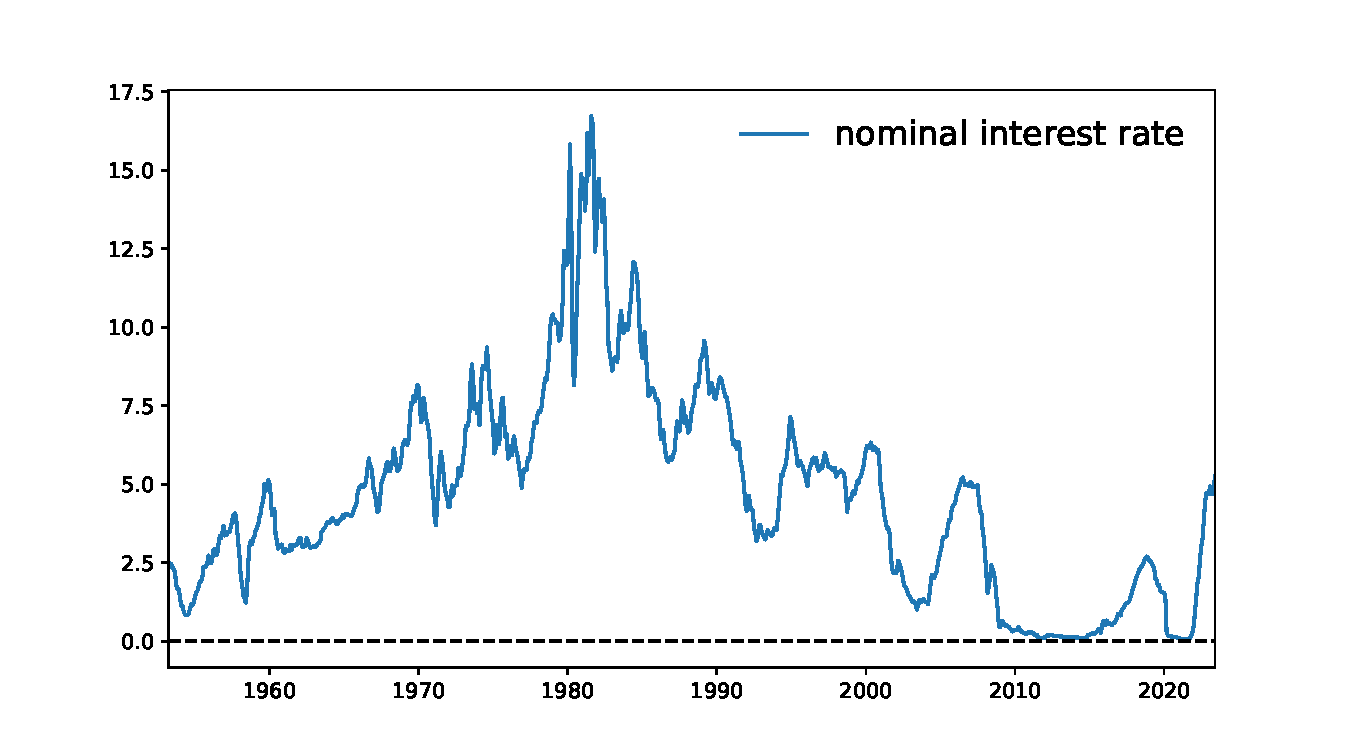
\includegraphics{figures/plot_interest_rates_nominal.pdf}}
       \caption{\label{f:plot_interest_rates_nominal} Nominal US interest rates}
    \end{figure}

\end{frame}

\begin{frame}
    
    \begin{figure}
       \centering
       \scalebox{0.4}{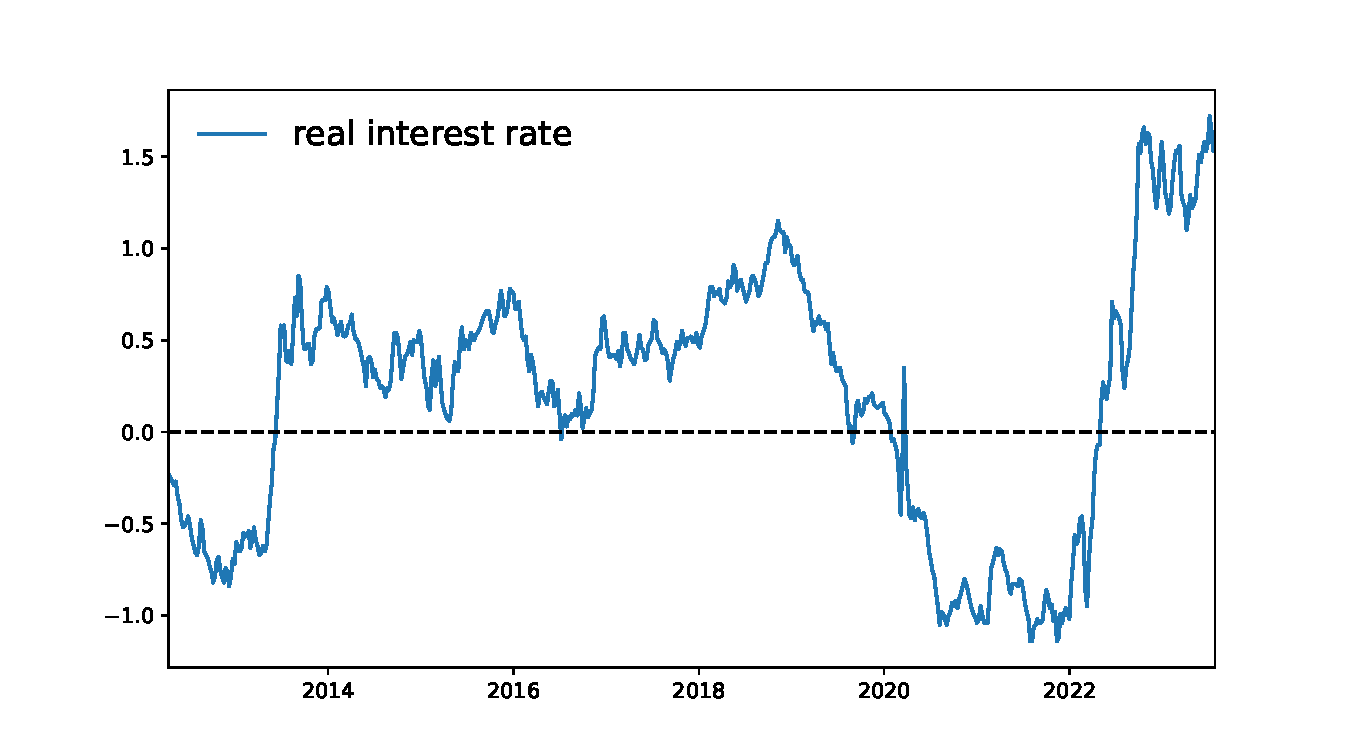
\includegraphics{figures/plot_interest_rates_real.pdf}}
       \caption{\label{f:plot_interest_rates_real} Real US interest rates
           }
    \end{figure}

\end{frame}


\begin{frame}
    
    Let's shift to a setting with state-dependent discounting

    \vspace{0.4em}
    \Eg Discount time $t$ reward $r_t$ via
    %
    \begin{equation*}
        \text{current value } = \EE \, \beta_1 \, \beta_2 \, \cdots  \,\beta_t \, r_t
    \end{equation*}

    \vspace{0.4em}
    \vspace{0.4em}
    \vspace{0.4em}

    Strategy:
    %
    \begin{enumerate}
        \item study computation of lifetime values under state-dependent
            discounting
        \vspace{0.4em}
        \item learn how to optimize these values across feasible policies
        \vspace{0.4em}
    \end{enumerate}


    Let's start with step 1:

\end{frame}



\begin{frame}
    \frametitle{Valuation with non-constant discounting}

    Let $(X_t)_{t \geq 0}$ be a state process 
    %
    \begin{itemize}
        \item the discount factor varies with $X_t$
        \vspace{0.4em}
        \item profits / payoffs vary with $X_t$
    \end{itemize}

        \vspace{0.4em}
        \vspace{0.4em}

    To construct the state process, we
    %
    \begin{itemize}
        \item let $\Xsf$ be finite and let $P$ be a Markov matrix on $\Xsf$:
            %
            \begin{equation*}
                P \geq 0
                \quad \text{and} \quad
                \sum_{x' \in \Xsf} P(x, x') = 1
            \end{equation*}
        \item let $(X_t)_{t \geq 0}$ be $P$-Markov on $\Xsf$:
        %
        \begin{equation*}
            \PP\{X_{t+1} = x' \given X_t = x\}
            = P(x, x')
        \end{equation*}
    \end{itemize}


\end{frame}

\begin{frame}
    
    Consider the \navy{discount factor process} 
    %
    \begin{equation*}
        \delta_t := \prod_{i=1}^t b(X_{i-1}, X_i) 
    \end{equation*}
    %
    \vspace{0.4em}

    \begin{itemize}
        \item \Eg $b \equiv \beta \in (0, 1)$ implies $\delta_t = \beta^t$ (const.\
            discounting)
        \vspace{0.4em}
        \item Assume $b > 0$
    \end{itemize}

    \vspace{0.4em}
    \vspace{0.4em}
    \vspace{0.4em}

    Let $A$ be the \navy{discount operator}
    %
    \begin{equation*}
        A(x,x') 
        := b(x, x') P(x, x') 
    \end{equation*}
    
    Let 
    %
    \begin{equation*}
        \rho(A) = \max_{\lambda \in \sigma(A)} |\lambda|,
        \qquad
        \sigma(A) := \text{ eigenvalues of } A
    \end{equation*}


\end{frame}



\begin{frame}\label{slide:gdr}

    Let $\RR^\Xsf =$ all real-valued functions on $\Xsf$
    %
        \vspace{0.4em}
        \vspace{0.4em}

    \begin{block}{\vspace*{-3ex}}
    {\bf Theorem.} If $h \in \RR^\Xsf$ and $\rho(A)<1$, then 
    %
    \vspace{0.4em}
    \begin{equation*}
        v(x) :=
            \EE_x \,
                \sum_{t=0}^\infty \, \delta_t \, h(X_t)
                \text{ is finite for all $x \in \Xsf$}
    \end{equation*}
    %

    \vspace{0.4em}
    \vspace{0.4em}
    Moreover, $I-A$ is bijective and 
    %
    \begin{align*}
        v  
        & = \sum_{t \geq 0} A^t h 
        \\
        & = (I - A)^{-1} h 
    \end{align*}
    %
    \end{block}

\end{frame}


\begin{frame}
    

    \underline{Sketch of proof}:  An inductive argument shows that

    \begin{equation*}
        \EE_x \, \delta_t \, h(X_t) = (A^t h)(x)
    \end{equation*}

    Hence
    %
    \begin{equation*}
        v(x) 
            = \EE_x \,
                \sum_{t=0}^\infty \, \delta_t \, h(X_t)
            = \sum_{t=0}^\infty \, \EE_x \, \delta_t \, h(X_t)
            = \sum_{t=0}^\infty \, (A^t h)(x)
    \end{equation*}

    That is, $v = \sum_{t \geq 0} A^t h$

        \vspace{0.4em}
        \vspace{0.4em}
        \vspace{0.4em}

    By $\rho(A) < 1$ and the Neumann series lemma,
    %
    \begin{equation*}
        \sum_{t \geq 0} A^t = (I - A)^{-1}
    \end{equation*}


\end{frame}

\begin{frame}
    
    Note that the condition $\rho(A) < 1$ is weak

    \begin{itemize}
        \item necessary as well as sufficient for convergence in many settings
        \vspace{0.5em}
        \item permits discount factor $>1$ with positive probability
    \end{itemize}

        \vspace{0.5em}
        \vspace{0.5em}
    The last fact means
    %
    \begin{itemize}
        \item can handle negative interest rates
        \vspace{0.5em}
        \item can handle models with large preference shocks
        \begin{itemize}
            \vspace{0.5em}
            \item ZLB literature
            \vspace{0.5em}
            \item asset pricing literature
        \end{itemize}
    \end{itemize}

\end{frame}





\begin{frame}

    Next steps

    \begin{enumerate}
        \item Obtain general results on DP with state-dependent
            discounting
        \vspace{0.4em}
        \vspace{0.4em}
        \item Apply them to the inventory problem
        \vspace{0.4em}
        \vspace{0.4em}
        \item Solve with Python / Julia using different algorithms
    \end{enumerate}

        \vspace{0.4em}
        \vspace{0.4em}
        \vspace{0.4em}
        \vspace{0.4em}
        \vspace{0.4em}

    Our general results will use the theorem on slide~\ref{slide:gdr}

    \begin{itemize}
        \item a condition to ensure that valuations are finite
    \end{itemize}

\end{frame}


\begin{frame}
    \frametitle{MDPs with State-Dependent Discounting}
    
    We consider a Markov decision process (MDP) with Bellman equation
    %
    \begin{equation*}
        v(x) =
        \max_{a \in \Gamma(x)}
        \left\{
            r(x, a) + \sum_{x'} v(x') \beta(x, a, x') P(x, a, x')
        \right\}
    \end{equation*}
    %
    for all $x \in \Xsf$

    \vspace{0.4em}
    \begin{itemize}
        \item $\Xsf, \Asf$ finite state \& action spaces
    \vspace{0.4em}
        \item $\Gamma$ a nonempty correspondence from $\Xsf \to \Asf$
    \vspace{0.4em}
        \item $\Gsf :=$ all $(x,a)$ s.t.\ $a \in \Gamma(x)$
    \vspace{0.4em}
        \item $\beta$ maps $\Gsf \times \Xsf$ to $(0, \infty)$
    \end{itemize}
\end{frame}

\begin{frame}
    
    Let $\Sigma$ be the set of \navy{feasible policies} 

    \begin{equation*}
        \Sigma 
        := \setntn{ \sigma \in \Asf^\Xsf }
        {\sigma(x) \in \Gamma(x) \text{ for all } x \in \Xsf}
    \end{equation*}

    Let 
    %
    \begin{itemize}
        \item $r_\sigma(x) := r(x, \sigma(x)) =$  rewards under $\sigma$
        \vspace{0.4em}
        \item $P_\sigma(x, x') := P(x, \sigma(x), x') =$ transitions under
            $\sigma$
        \vspace{0.4em}
        \item $\beta_\sigma(x, x') := \beta(x, \sigma(x), x') =$ discounting under
            $\sigma$
    \end{itemize}
        


    \vspace{0.4em}
    \vspace{0.4em}
    \vspace{0.4em}
    Note that $P_\sigma$ is Markov dynamics for the state under $\sigma$


\end{frame}

\begin{frame}
    

    When it exists, the \navy{lifetime value} $v_\sigma$ of $\sigma$ obeys
    %
    \begin{equation*}
        v_\sigma(x)
        = \EE_x \sum_{t=0}^\infty \delta_t^\sigma \, r_\sigma(X_t)
    \end{equation*}
    %
    where 
    %
    \begin{equation*}
        \delta_t^\sigma := 
        \prod_{i=1}^t \beta_\sigma(X_{i-1}, X_i)
    \end{equation*}
    %
    and 
    %
    \begin{center}
         $(X_t)_{t \geq 0}$ is $P_\sigma$-Markov with $X_0 = x$
    \end{center}

\end{frame}


\begin{frame}
    
    Let 
    %
    \begin{equation*}
        L_\sigma(x,x') := \beta_\sigma(x, x') P_\sigma(x, x')
    \end{equation*}

            \vspace{0.4em}
            \vspace{0.4em}

    \begin{block}{\vspace*{-3ex}}
        {\bf Proposition.} If $\rho(L_\sigma) < 1$, then 
        %
            \vspace{0.4em}
        \begin{itemize}
            \item $I - L_\sigma$ is bijective
            \vspace{0.4em}
            \item $v_\sigma$ is finite and 
                $$
                v_\sigma = \sum_{t \geq 0} L_\sigma^t r_\sigma = (I - L_\sigma)^{-1} r_\sigma
                $$
        \end{itemize}
        %
    \end{block}

            \vspace{0.4em}
            \vspace{0.4em}
            \vspace{0.4em}
    \underline{Proof}: Follows directly from the result on slide~\ref{slide:gdr}

\end{frame}


\begin{frame}

    Let $T_\sigma$ be the \navy{policy operator} corresponding to $\sigma$:
    %
    \begin{equation*}
        T_\sigma \, v := r_\sigma + L_\sigma \, v
    \end{equation*}


    Note that 
    %
    \begin{align*}
        v_\sigma 
        & = (I - L_\sigma)^{-1} r_\sigma
        \\
        & \iff \quad
            v_\sigma \text{ solves eq. } (I - L) v =  r_\sigma 
            \\
        & \iff \quad
            v_\sigma \text{ solves eq. } v =  r_\sigma + L_\sigma v
            \\
        & \iff \quad
            v_\sigma \in \fix(T_\sigma)
    \end{align*}

    \vspace{0.4em}
    
    %
    By the results on slide~\ref{slide:gdr},
    %
    \begin{equation*}
        \rho(L_\sigma) < 1
        \implies 
        \fix(T_\sigma) = \{v_\sigma\}
    \end{equation*}


\end{frame}


\begin{frame}
    
    \Fact $T_\sigma$ is \navy{globally stable} on $\RR^\Xsf$ when $\rho(L_\sigma) <
    1$:
    %
    \begin{equation}\label{eq:gs}
        \forall  \, v \in \RR^\Xsf,
        \qquad
        T_\sigma^k v \to v_\sigma
        \quad \text{ as } \quad k \to \infty
    \end{equation}

    \begin{itemize}
        \item See proof in \url{https://dp.quantecon.org/}
    \end{itemize}
    \vspace{0.4em}
    \vspace{0.4em}
    \vspace{0.4em}
    Hence we have three ways to compute $v_\sigma$:

    \vspace{0.4em}
    \vspace{0.4em}
    \begin{enumerate}
        \item $ v_\sigma = \sum_{t \geq 0} L_\sigma^t r_\sigma$
    \vspace{0.4em}
        \item  $v_\sigma = (I - L_\sigma)^{-1} r_\sigma$
    \vspace{0.4em}
        \item via \eqref{eq:gs}
    \end{enumerate}

\end{frame}


\begin{frame}

    We need a uniform bound, for all $\sigma \in \Sigma$:
    %

    \vspace{0.4em}
    \vspace{0.4em}
    \begin{block}{\vspace*{-3ex}}
        {\bf Proposition.} If $\exists$ an $L$ such that 
        %
            \vspace{0.4em}
        \begin{itemize}
            \item $L_\sigma \leq L$ for all $\sigma \in \Sigma$
            \vspace{0.4em}
            \item $\rho(L) < 1$
        \end{itemize}
        % 
        \vspace{0.4em}
        then, for all $\sigma \in \Sigma$, the unique fixed point of $T_\sigma$
        in $\RR^\Xsf$ is
        %
        \begin{equation*}
            v_\sigma = (I - L_\sigma)^{-1} r_\sigma
        \end{equation*}
        %
    \end{block}

    
        \vspace{0.4em}
    \underline{Proof}: Immediate from 
    %
    \begin{enumerate}
        \item $0 \leq A \leq B$ implies $\rho(A) \leq \rho(B)$
        \vspace{0.4em}
        \item $0 \leq L_\sigma \leq L$ and $\rho(L) < 1$
    \end{enumerate}

\end{frame}



\begin{frame}
    
    What we have achieved

    \begin{itemize}
        \item found a condition for finite lifetime values across all policies
        \vspace{0.4em}
        \item found methods to compute these lifetime values
    \end{itemize}


        \vspace{0.4em}
        \vspace{0.4em}
        \vspace{0.4em}
        \vspace{0.4em}
    Yet to do

    \begin{itemize}
        \item show how to maximize lifetime values across $\sigma \in \Sigma$
        \vspace{0.4em}
        \item implement numerically
    \end{itemize}

\end{frame}


\begin{frame}
    \frametitle{Defining optimality}
    
    Suppose the stated condition holds
    %
    \begin{itemize}
        \item $\exists$ matrix $L$ with $\rho(L) < 1$ and $L_\sigma \leq L$ for
            all $\sigma$
    \end{itemize}

    \vspace{0.4em}
    \vspace{0.4em}
    Then $v_\sigma$ is finite for all $\sigma$

    \vspace{0.4em}
    \vspace{0.4em}
    Hence we can define the \navy{value function} 
    
    \begin{equation*}
        v^*(x) := \max_{\sigma \in \Sigma} v_\sigma(x)
        \quad \qquad (x \in \Xsf)
    \end{equation*}

    \vspace{0.4em}
    \vspace{0.4em}
    \vspace{0.4em}
    \vspace{0.4em}
    A policy $\sigma$ is called \navy{optimal} if $v_\sigma = v^*$


\end{frame}



\begin{frame}
    
    The \navy{Bellman operator} takes the form
    %
    \begin{equation*}
        (Tv)(x) = \max_{a \in \Gamma(x)}
            \left\{
            r(x, a) + \sum_{x'} v(x') \beta(x, a, x') P(x, a, x')
        \right\}
    \end{equation*}
    

    \vspace{0.4em}
    \vspace{0.4em}

    \vspace{0.4em}
    Given $v \in \RR^\Xsf$, a policy $\sigma$ is called \navy{$v$-greedy} if 
    %
    \begin{equation*}
        \sigma(x) \in \argmax_{a \in \Gamma(x)}
        \left\{
            r(x, a) + \sum_{x'} v(x') \beta(x, a, x') P(x, a, x')
        \right\}
    \end{equation*}

     for all $x$ in $\Xsf$



\end{frame}



\begin{frame}\label{slide:sdd_op}

    \begin{block}{\vspace*{-3ex}}
    {\bf Proposition.} If there exists a linear operator $L$ on $\RR^\Xsf$ such
    that 
    %
    \begin{equation*}
        \rho(L)<1
        \quad \text{and} \quad
        \beta(x, a, x') P(x, a, x') \leq L(x, x')
    \end{equation*}
    %
    for all $(x,a) \in \Gsf$ and $x' \in \Xsf$, then 
    %
    \vspace{0.4em}
    \vspace{0.4em}
    \begin{enumerate}
        \item $T_\sigma$ is globally stable on
            $\RR^\Xsf$ with unique fixed point $v_\sigma$
    \vspace{0.4em}
    \vspace{0.4em}
        \item $v_\sigma = (I - L_\sigma)^{-1} r_\sigma$
    \vspace{0.4em}
    \vspace{0.4em}
        \item $T$ is globally stable on
            $\RR^\Xsf$ with unique fixed point $v^*$
    \vspace{0.4em}
    \vspace{0.4em}
        \item a policy $\sigma \in \Sigma$ is optimal if and only if it is
            $v^*$-greedy
    \vspace{0.4em}
    \vspace{0.4em}
        \item at least one optimal policy exists
    \end{enumerate}
    %
    \end{block}

\end{frame}



\begin{frame}
    \frametitle{Algorithms}


    Now we have 
    %
    \begin{itemize}
        \item conditions for optimality
        \vspace{0.4em}
        \item general DP optimality results
    \end{itemize}


        \vspace{0.4em}
        \vspace{0.4em}
    Next we need algorithms 

        \vspace{0.4em}

    Let's consider
    
    \begin{itemize}
        \item value function iteration (VFI)
        \vspace{0.4em}
        \item Howard policy iteration (HPI)
        \vspace{0.4em}
        \item  optimistic policy iteration (OPI)
    \end{itemize}


\end{frame}



\begin{frame}
    
    {\small 
        \begin{algorithm}[H]
        \DontPrintSemicolon
        \vspace{0.2em}
        input $v_0 \in \RR^\Xsf$ \;
        \vspace{0.2em}
        input $\tau$, a tolerance level for error \;
        \vspace{0.2em}
        $\epsilon \leftarrow +\infty$ \;
        \vspace{0.2em}
        $k \leftarrow 0$ \;
        \vspace{0.2em}
        \While{$\epsilon > \tau $}
        {
        \vspace{0.2em}
            $v_{k+1} \leftarrow Tv_k$ \;
            \vspace{0.2em}
            $\epsilon \leftarrow \| v_k - v_{k+1} \|_\infty$ \;
            \vspace{0.2em}
            $k \leftarrow k + 1$ \;
        \vspace{0.2em}
        }
        \vspace{0.2em}
        Compute a $v_k$-greedy policy $\sigma$ \;
        \vspace{0.2em}
        \Return{$\sigma$}
        \vspace{0.2em}
        \caption{VFI}
        \end{algorithm}
    }

\end{frame}



\begin{frame}
    
    \begin{algorithm}[H]
        \DontPrintSemicolon
        input $\sigma_0 \in \Sigma$, an initial guess of $\sigma^*$ \;
        \vspace{0.4em}
        $k \leftarrow 0$ \;
        \vspace{0.4em}
        $\epsilon \leftarrow +\infty$ \;
        \vspace{0.4em}
        \While{$\epsilon > 0 $}
        {
            $v_k \leftarrow (I - L_{\sigma_k})^{-1} r_{\sigma_k}$ \;
            \vspace{0.4em}
            $\sigma_{k+1} \leftarrow $ a $v_k$-greedy policy \;
            \vspace{0.4em}
            $\epsilon \leftarrow \1 \{ \sigma_k \not= \sigma_{k+1} \}$ \;
            \vspace{0.4em}
            $k \leftarrow k + 1$ \;
        }
            \vspace{0.4em}
        \Return{$\sigma_k$}
        \caption{\label{algo:hpi_sd} HPI}
    \end{algorithm}

\end{frame}


\begin{frame}
    
    \begin{figure}
       \begin{center}
        \input{flint.tex}
        %\vspace{1em}
        %\caption{\label{f:flint} HPI}
       \end{center}
    \end{figure}


\end{frame}
    

\begin{frame}
    
    \begin{figure} 
        \centering
        \scalebox{0.48}{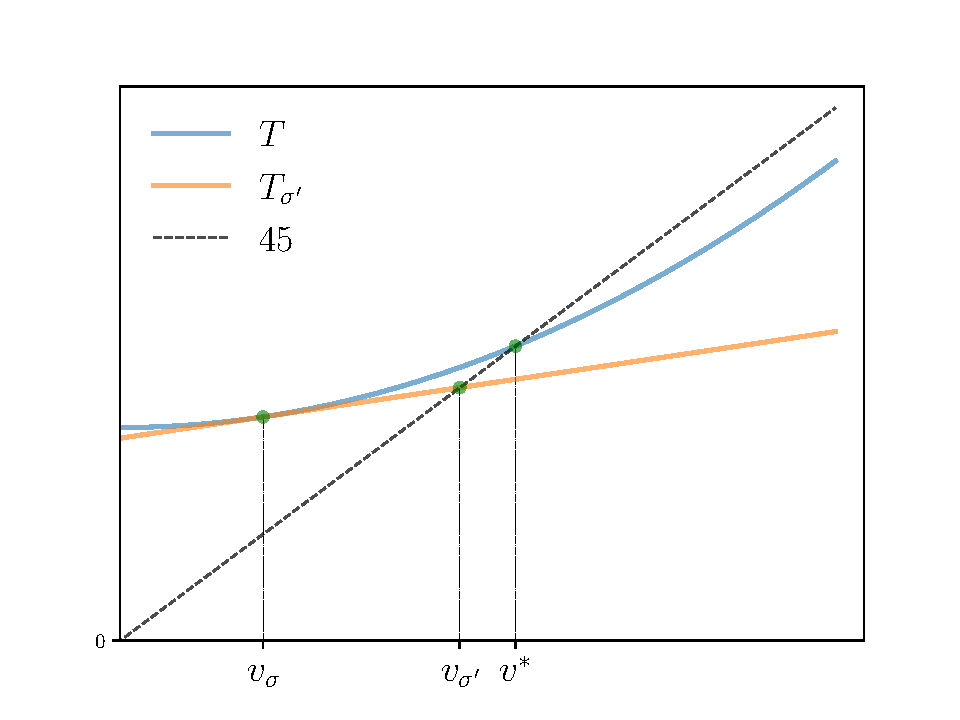
\includegraphics{howard_newton_1.pdf}}
        \caption{\label{f:howard_newton_1} HPI as a version of Newton's method}
    \end{figure}
    %

\end{frame}

\begin{frame}
    
    {\small
    \begin{algorithm}[H]
        \DontPrintSemicolon
        \vspace{0.2em}
        input $v_0 \in \RR^\Xsf$, an initial guess of $v^*$ \;
        \vspace{0.2em}
        input $\tau$, a tolerance level for error \;
        \vspace{0.2em}
        input $m \in \NN$, a step size \;
        \vspace{0.2em}
        $k \leftarrow 0$ \;
        \vspace{0.2em}
        $\epsilon \leftarrow +\infty$ \;
        \vspace{0.2em}
        \While{$\epsilon > \tau $}
        {
            \vspace{0.2em}
            $\sigma_k \leftarrow $ a $v_k$-greedy policy \;
            \vspace{0.2em}
            $v_{k+1} \leftarrow T_{\sigma_k}^m v_k$  \;
            \vspace{0.2em}
            $\epsilon \leftarrow \| v_k - v_{k+1} \|_\infty$ \;
            \vspace{0.2em}
            $k \leftarrow k + 1$ \;
            \vspace{0.2em}
        }
        \Return{$\sigma_k$}
        \vspace{0.2em}
        \caption{OPI}
    \end{algorithm}
    }

\end{frame}


\begin{frame}
    
    \vspace{0.4em}
    \vspace{0.4em}
    \vspace{0.4em}
    \begin{block}{\vspace*{-3ex}}
    {\bf Proposition.} Under the stated condition, VFI, HPI and OPI all converge
    \vspace{0.4em}
    \vspace{0.4em}

    Moreover, HPI converges to an exact optimal policy in finitely many steps
    \end{block}


    \vspace{0.4em}
    \vspace{0.4em}
    For details and proofs see Ch.\ 6 of \url{https://dp.quantecon.org/}


\end{frame}



\begin{frame}
    \frametitle{Back to the inventory problem}

    Replace $\beta$ with $\beta(Z_t)$ where 
        $(Z_t)_{t \geq 0}$ is $Q$-Markov on $\Zsf$

    \vspace{0.5em}
    The Bellman equation becomes
    %
    \begin{equation*}
         v(y, z) =
         \max_{a \in \Gamma(y)}
         \left\{
             r(y, a) + \beta(z) 
                 \sum_{z', \; y'}
                v(y', z') Q(z, z') R(y, a, y')
            \right\}
    \end{equation*}
    %

    \vspace{0.5em}
    Given $\sigma \in \Sigma$, the \navy{policy operator} is
    %
    \begin{multline*}
        (T_\sigma \, v)(y, z) =
             r(y, \sigma(y, z)) + 
             \\
             \beta(z) 
             \sum_{z' , \; y'}
                v(y', z') Q(z, z') R(y, \sigma(y, z), y')
    \end{multline*}
    %


\end{frame}



\begin{frame}


    \begin{block}{\vspace*{-3ex}}

    {\bf Proposition} 
    Let
    %
    $$L(z, z') := \beta(z) Q(z, z')$$

    \vspace{0.5em}
    If $r(L)<1$, then all of the optimality results on slide~\ref{slide:sdd_op}
    apply

    \end{block}

    \vspace{0.5em}
    \vspace{0.5em}

    \Ex Check the details

    \vspace{0.5em}
    \vspace{0.5em}
    \vspace{0.5em}
    \begin{itemize}
        \item See Ch.\ 6 of \url{https://dp.quantecon.org/} if you get stuck
    \end{itemize}

\end{frame}





\begin{frame}
    

    Code that solves the model can be found at

    \begin{itemize}
        \item \url{https://github.com/QuantEcon/dse_2023}
    \end{itemize}

    \vspace{0.5em}
    \vspace{0.5em}
    \vspace{0.5em}
    Illustrates

    \begin{itemize}
        \item Python vs Julia
        \vspace{0.5em}
        \item Numba vs NumPy vs JAX
        \vspace{0.5em}
        \item Power of GPUs --- if you have one
    \end{itemize}

\end{frame}




\end{document}









